\chapter{Merging algorithm}
\label{chap:mergingalgorithm}

In this chapter we present an merging algorithm based on computer vision techniques. This is not completely new even in \gls{ROS} environment. First computer vision-based approach to merging was implemented in~\cite{MapstitchROS}. This package's primary purpose was to stitch generated map to existing static map.

Although this package was not developed for map merging in multi-robot configuration, algorithm and its original implementation were used for coordinated multi-robot exploration solution presented in~\cite{Andre2014}.

Due to its original purpose, mapstitch algorithm shows some limitations for multi-robot map merging setup. Originally it was designed for offline use~\cite{Andre2014}. Also, it was designed for stitching two maps, one them being large reference map covering most of the environment. Although it is possible to incrementally merge maps from multiple robots with this algorithm, global map quality generally decreases with increasing number of robots. Significant decrease in performance was observed for 4 robots~\cite{Andre2014}.

\begin{algorithm}
    \caption{Mapstitch original algorithm}
    \label{alg:mapstitch}
    \begin{algorithmic}[1]
        \Require $2$ occupancy grids
        \Ensure transformation between $2$ grids
        \Procedure{StitchedMap}{$grid1, grid2$}
            \State detect \gls{ORB} features
            \State match keypoints with Brute-Force matcher
            \State find matching point pairs with same distance in both images
            \State find homography (affine transform)
        \EndProcedure
    \end{algorithmic}
\end{algorithm}

Algorithm~\ref{alg:mapstitch} shows original algorithm used in~\cite{MapstitchROS}, version used in~\cite{Andre2014} is only a slightly modified.

Although our algorithm also uses computer vision-based approach, proposed algorithm deals with most of the limitations of the original simple algorithm. Proposed algorithm is designed to work with unlimited number of grids, so there is no additional need for iterative merging. More importantly, by design, algorithm can determine optimal order of individual pairwise merges. I assume this might be the main reason for decrease in performance in $4$-robot setup observed by~\cite{Andre2014}. Also proposed algorithm deals with other problems arising for general $n$-map merge problem such as situations when it is not possible to merge some of the maps because transformation to others could not be reliably estimated, cases where map transformation can be estimated from more sources (multiple neighbours) etc.

\section{Stitching pipeline} % (fold)
\label{sec:stitchingpipeline}

As discussed in chapter \#reference here\# our algorithm is inspired by image stitching algorithms. Stitching algorithms are well-understood and implementations are broadly available. General concept of multi-step stitching pipeline is described in~\cite{Brown2006}. Stitching pipeline is also well established code in \gls{OpenCV}, mostly based on~\cite{Brown2006}, along with~\cite{Szeliski2004} \cite{Shum1998} and others. Figure~\ref{fig:opencv} highlights processing steps in stitching as implemented in \gls{OpenCV}.

\begin{figure}
	\centering
	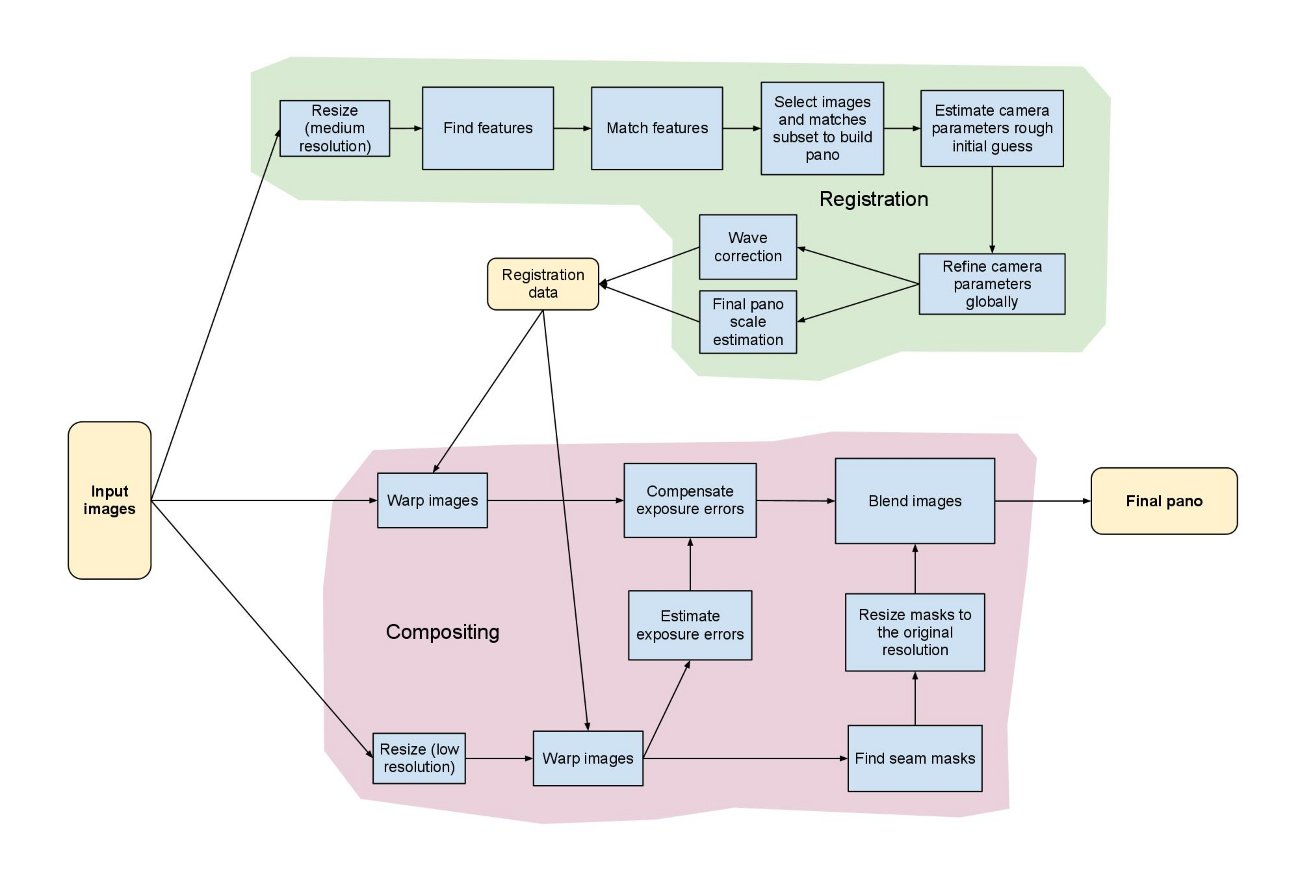
\includegraphics[width=4.33in]{../img/StitchingPipeline.jpg}
	\caption{\gls{OpenCV} Stitching pipeline.}
	\label{fig:opencv}
\end{figure}

Our algorithm will solve the registration part of stitching according to figure~\ref{fig:opencv}. As compositing part of stitching is relatively simple for occupancy grids compared to images from camera, because we don't need to compensate exposure errors, gain and other deficiencies. This solves the main problem of acquiring transformation between robots individual frames and bridging the problem of merging maps with known initial positions and unknown initial positions.

\gls{ROS} node for map merging described in \#reference here\# implements also compositing part of the pipeline, which is simple when transformation is estimated with high precision.

For description of the algorithm we will assume to have maps represented as occupancy grids, with each cell containing value in range $[0,100]$ indicating probability that there is obstacle in the cell and $-1$ for indicating unknown probability. This representation is basically greyscale image, hence using image processing algorithms seems natural.

We will consider occupancy grids greyscale images through algorithm~\ref{alg:estimategridtrasform}. Values in the image are exactly the same is in occupancy grids, without any mapping. This means images are be basically only $7$-bit depth.

Algorithm~\ref{alg:estimategridtrasform} offers overview of the proposed algorithm, detailed description will be provided in following sections.

\begin{algorithm}
    \caption{Proposed algorithm for estimating transform between multiple occupancy grids}
    \label{alg:estimategridtrasform}
    \begin{algorithmic}[1]
        \Require occupancy grids
        \Ensure for each grid: transformation between grid and global reference frame, or value indicating transformation could not be be estimated for current grid
        \Procedure{estimateGridTransform}{$grids$}
            \State detect \gls{ORB} features (keypoints) for each grid
            \ForAll{pair of grids} \Comment{we will compute transformation between each image along with confidence}
            	\State match features
            	\State $n \gets \text{number of matches}$
            	\If{$n \le \text{matches threshold}$}
            		\State confidence $\gets 0$
            	\Else
            		\State find restricted affine transformation for keypoints using \gls{RANSAC}
            		\State $\psi \gets \text{number of inliers in \gls{RANSAC}}$
            		\If{transformation found}
            			\State confidence $\gets \frac{\psi}{8 + 0.3 \cdot n}$
            		\Else
            			\State confidence $\gets 0$
            		\EndIf
            	\EndIf
            \EndFor
            \State matches $\gets (i,j)$ for matches with confidence $\ge 1.0$
            \State $g \gets (grids, matches)$
            \State $h \gets$ largest connected component in $g$
            \State $t \gets$ maximum spanning tree in $h$
            \State walk $t$ and compute transformations to global reference frame
        \EndProcedure
    \end{algorithmic}
\end{algorithm}

% section stitching_pipeline (end)

\section{Feature detection} % (fold)
\label{sec:featuredetection}

Stitching pipeline proposed in \cite{Brown2006} is using \gls{SIFT} features. \gls{SIFT} features have been used with success for stitching in many applications. Some of the recent approaches to stitching, improving traditional \gls{SIFT}-based algorithm, are also building on top of \gls{SIFT} features \cite{Xie2015}. \gls{SIFT} features are patented in the US \cite{lowe2004method}, limiting its use.

I have decided to use \gls{ORB} as feature detector a descriptor described in \cite{Rublee2011}. \gls{ORB} algorithm is patent-free, and available in \gls{OpenCV}. \gls{ORB} features has been already used with occupancy grid images \cite{MapstitchROS} \cite{Andre2014}.

Other alternatives for feature detection and feature description has not been tested yet. Performance of other detectors for map merging and effect of choose of detector to overall merging performance remains to be evaluated. Some feature detectors and descriptors promising good performance are \cite{Alahi2012} \cite{alcantarilla2011fast} \cite{calonder2010brief}.

For image stitching, images are usually downscaled for further processing as seen is figure~\ref{fig:opencv}. Feature extraction and feature matching on smaller images is considerably faster and final performance is acceptable. I don't propose any such down scaling for occupancy grids. Occupancy grids acquired from mapping are usually smaller than multi-megapixel images from camera, so stitching time is reasonable even for full-scale grids. Also occupancy grids have usually much smaller number of features than photos making stitching harder and less precise.

During online merging we can run stitching with low frequency even if higher map update frequencies are required by simply using previously estimated transform between grids. This further reduces cost of estimation over time. Since transformation between grids is fixed in most cases (when \gls{SLAM} algorithm work reasonably well), depending only on starting points of robots, this approach does not reduce map quality considerably.

In most tested scenarios estimated transformation change only during initial phase. After there is enough overlapping regions in the map, such that transformation can be estimated with enough precision, transformation estimated with stitching algorithm remains stable over time. This property allows to run re-estimation with low frequencies.

% section feature_detection (end)

\section{Pairwise matching} % (fold)
\label{sec:pairwisematching}

Pairwise matching is the most resource demanding part of the algorithm. We do matching for all $\bigO(n^2)$ pairs of grids. For panorama images it is possible to push this down to $\bigO(n)$ matching by expecting photos to be taken in ordered sequence. We can then match image only $k$ neighbours (for small $k$) in sequence, because neighbours are expected to have overlapping area.

For occupancy grids in multi-robot mapping scenario it is impractical to assume any such ordering in robot's initial poses. It might not even be possible when robots are exploring given areas independently. Our algorithm therefore always match all $\bigO(n^2)$ pairs.

Because computations in each pair are independent it is easy to run matching of all pairs in parallel or offload it GPU. This approach is used in map merging node presented in \#reference here\#.

\begin{figure}
    \centering
    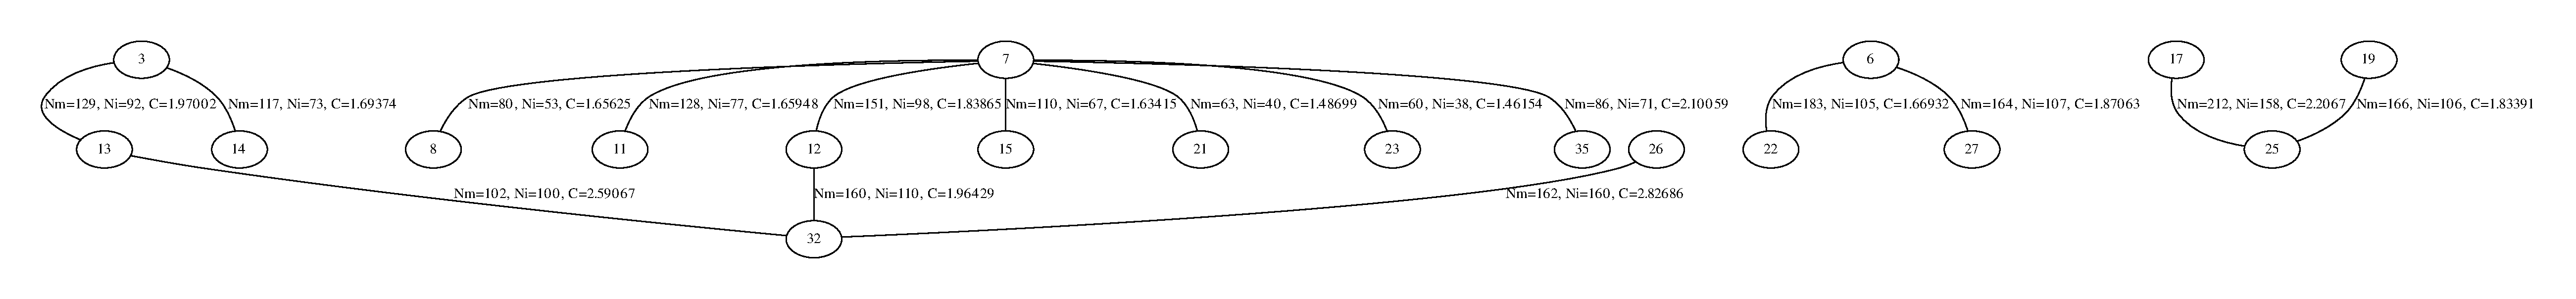
\includegraphics[width=\textwidth]{../img/matches.pdf}
    \caption{Graph showing matches between $37$ occupancy grids during map merging. This graph was acquired for maps from MIT dataset, see chapter \#reference here\#. Grids without any matches are omitted. Legend: $Nm$ number of matches, $Ni$ number of inliers from \gls{RANSAC}, $C$ confidence.}
    \label{fig:matches}
\end{figure}

Figure~\ref{fig:matches} shows matching results for $37$ occupancy grids acquired during experiment \#reference here\#.

Because of non-linear number of pairs it is usually too computationally expensive to search for matches using simple (brute-force) search unless this can be offloaded to GPU. For matching on CPU it is better to use approximate methods, which can be much faster.

For vector-based features, such as \gls{SIFT} and \gls{SURF}, the solution has been to use approximate nearest-neighbour search, but these existing algorithms are not suitable for binary features \cite{Muja2012}. For \gls{ORB} features, which are binary based, searching for nearest neighbours using parallel hierarchical clustering trees proposed in \cite{Muja2012} can provide similar speed-up for \gls{ORB} features. This method is used through the \gls{FLANN} by the same authors, which is now part of \gls{OpenCV}.

When matching keypoints are found for pair of grids, algorithm estimates transformation between grids. Traditional image stitching algorithms are using homography in projective spaces, which is a good for modelling perspective affecting camera images. For occupancy grids this is not an expected transformation under normal circumstances, and even when there are errors in maps produced by \gls{SLAM} algorithm, these are not errors produced by projective transformation.

For occupancy grids we propose a different model based on reduced affine transform. This is a partial affine transformation with $4$ degrees of freedom.

\begin{defn}[Reduced affine transformation]
For given matrices $R$ (rotation), $S$ (scaling), $T$ (translation), where

\begin{align}
    R &=
    \begin{pmatrix}
        \cos{\theta} & -\sin{\theta} \\
        \sin{\theta} & \cos{\theta} \\
    \end{pmatrix} \\
    S &=
    \begin{pmatrix}
        s & 0 \\
        0 & s \\
    \end{pmatrix} \\
    T &=
    \begin{pmatrix}
        tx \\
        ty \\
    \end{pmatrix}
\end{align}

we define matrix of reduced affine transformation as

\begin{equation}
    A =
    \begin{pmatrix}
        RS|T
    \end{pmatrix}
    =
    \begin{pmatrix}
        \cos(\theta)s & -\sin(\theta)s & tx \\
        \sin(\theta)s & \cos(\theta)s & ty \\
    \end{pmatrix}
\end{equation}.
\end{defn}

As usual when representing translations we will work with reduced affine transformation in homogeneous coordinates, where this transformation is homomorphism. Therefore we extend $A$ as

\begin{equation}
    A' =
    \begin{pmatrix}
        \cos(\theta)s & -\sin(\theta)s & tx \\
        \sin(\theta)s & \cos(\theta)s & ty \\
        0 & 0 & 1 \\
    \end{pmatrix}
\end{equation}

to represent reduced affine transformation in homogeneous coordinates space.

For pair of matched points $X=\T{(x_1,x_2,1)}$, $Y=\T{(y_1, y_2, 1)}$ we can then solve

\begin{align}
    A'X &= Y \label{eq:affinetrans}\\
    \begin{pmatrix}
        \cos(\theta)s & -\sin(\theta)s & tx \\
        \sin(\theta)s & \cos(\theta)s & ty \\
        0 & 0 & 1 \\
    \end{pmatrix}
    \begin{pmatrix}
        x_1 \\
        x_2 \\
        1
    \end{pmatrix}
    &=
    \begin{pmatrix}
        y_1 \\
        y_2 \\
        1
    \end{pmatrix}
\end{align}

for $\T{(\cos(\theta)s, \sin(\theta)s, tx, ty)}$ to obtain transformation between grids. This is easy to solve and need only $2$ points to get the transformation.

Reduced affine transformation is chosen to model transformation between initial robot poses in $2D$ space. Each robot can start at different position and have different orientation in terms of rotation in $2D$ space. Scaling enables occupancy grids to have different resolution.

We combine~\eqref{eq:affinetrans} with \gls{RANSAC}~\cite{fischler1981random} method to obtain final transformation. \gls{RANSAC} is used to estimate homography in image stitching method proposed in~\cite{Brown2006}. We use the same method for estimating reduced affine transformation. Using \gls{RANSAC} has another advantage. We can used number of inliers in \gls{RANSAC} to estimate transformation accuracy.

For each pair we compute confidence as $\frac{\psi}{8 + 0.3 \cdot n}$, where $n$ is number of matches and $\psi$ is number of inliers in \gls{RANSAC}. Model for confidence is based on probabilistic model for image match verification proposed in~\cite{Brown2006}.

For \gls{RANSAC} I have chosen following parameters: maximum number of iterations $500$, good ratio $0.5$. Same parameters are used internally in \gls{OpenCV}. If maximum number of iteration is reached and transformation therefore could not be found, its confidence is set to $0$.

% section pairwise_matching (end)

\section{Finding largest connected component} % (fold)
\label{sec:findinglargestconnectedcomponent}

As seen in figure~\ref{fig:matches} it is common that not all transformations could be established between grids. Graph of matchings therefore can have multiple connected components. We need to deal with missing transformations between components to estimate transformations for grids.

We could include all components to resulting map and position them such they don't overlap. This setup would preserve all information, but resulting map can't be topologically correct. Another approach is to choose only one connected component for final merge. This approach preserves map's topological accuracy. I have chosen the latter approach.

As a next in the algorithm we filter out matches according to selected probabilistic model for accuracy. Matches with computed confidence $\le 1.0$ are not further considered for matching.

After matches are filtered largest component is found in matches graph. Transformation will be established only for grids in largest connected component.

Choosing largest connected component might seem natural, but this approach has its caveats. Largest connected component represents matches between largest number of robots, however maps from the largest number of robots does not need to represent largest area in the map. This might be a problem especially in systems with heterogeneous robots, where mapping performance differs greatly between robots. Also some parts of maps might be much harder for robots to explore and despite large number of robots in such an area, produced map may be smaller than map produced by other group of robots (represented in graph as smaller component).

Modifications of this algorithm might choose to find weighted largest connected component in matchings graph. Weight could be based on discovered area in each map, such that the largest weighted connected component would represent largest discovered area.

I have chosen to use unweighted largest connected component, because it is less computationally expensive (weighting grids to represent discovered area in each grid require visiting each cell of each grid). Algorithm using unweighted largest connected component provides good results for small number of robots \#reference here\#. Approach using weighted components needs to be evaluated for more robots and larger environments.

% section finding_largest_connected_component (end)

\section{Estimate final transformation} % (fold)
\label{sec:estimatefinaltransformation}

Remaining graph is connected and it is possible to estimate transformation for all grids. We have estimated transformations between pairs of grids, edges for some pairs may be missing, because they were filtered out in previous steps.

Final part of the algorithm estimates transformation to global reference frame for each grid. We can choose reference frame of one of the grids as global reference frame, because we are interested in relative transformations between all grids for merging. This will be the reference frame of merged map.

Selecting global reference frame is not enough, because there may exist multiple paths from grid selected as reference frame to other grids. We construct maximum spanning tree to break these cycles. Edges are weighted with number of inliers to prefer stronger matches. This approach is routinely used for image stitching, exactly the same construct is implemented in \gls{OpenCV}.

Finally we can walk through spanning tree to obtain final transforms. There is now only one path from grid selected as reference frame to other grids. For each grid we can get the final by compositing pairwise transformations along the path. As we are working in homogeneous coordinates this is equivalent to matrix product of pairwise transformations along the path. This can be done in linear time with algorithm~\ref{alg:estimatefinaltrans}.

\begin{algorithm}
    \caption{Algorithm estimating transformations to global reference frame from pairwise transformations on spanning tree.}
    \label{alg:estimatefinaltrans}
    \begin{algorithmic}[1]
        \Require $t$ maximum spanning tree on grids, $P_{(i,j)}$ is pairwise reduced affine transformation between grids $i, j$
        \Ensure $T_i \forall i \in V$ transformations
        \Procedure{estimateFinalTrasform}{$t = (V,E)$, $P_e \forall e \in e$}
            \State $e \gets$ edges of $t$ sorted by discover time in \gls{BFS} started from grid with reference frame \Comment{using \gls{BFS} or \gls{DFS} does not matter here}
            \State $\forall T_i: T_i \gets I$ \Comment{initialize transformations with identity}
            \ForAll{$(i,j)$ in $e$}
                $T_j \gets T_i P_{(i,j)}$
            \EndFor
        \EndProcedure
    \end{algorithmic}
\end{algorithm}

% section estimate_final_transformation (end)